Figures 1-6 show the intensity versus polarization with each separate graph respresenting the different solutions. Each of the graphs contain data for different beaker sizes (small, medium, large).

\begin{figure}[H]
    \begin{center}
        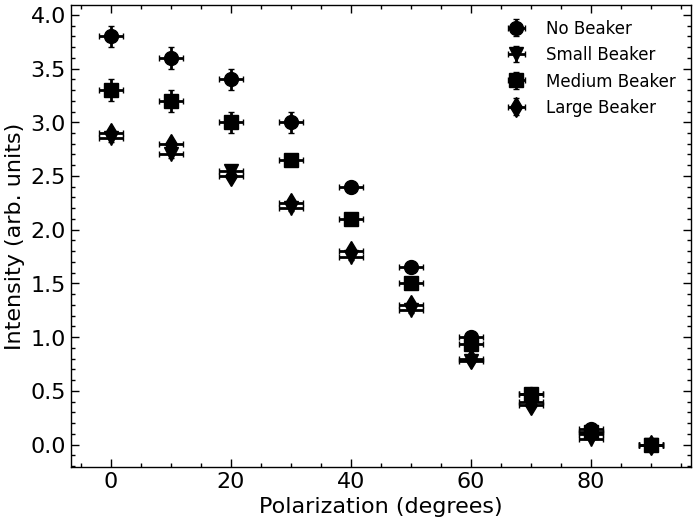
\includegraphics[width=\columnwidth]{../figures/no_water.png}
    \end{center}
    \caption{Intensity vs. Polarization for varying beaker sizes with no water. Here, the polarization is measured in degrees and the intensity is measured in arbitrary units.}
    \label{fig:no_water}
\end{figure}

\begin{figure}[H]
    \begin{center}
        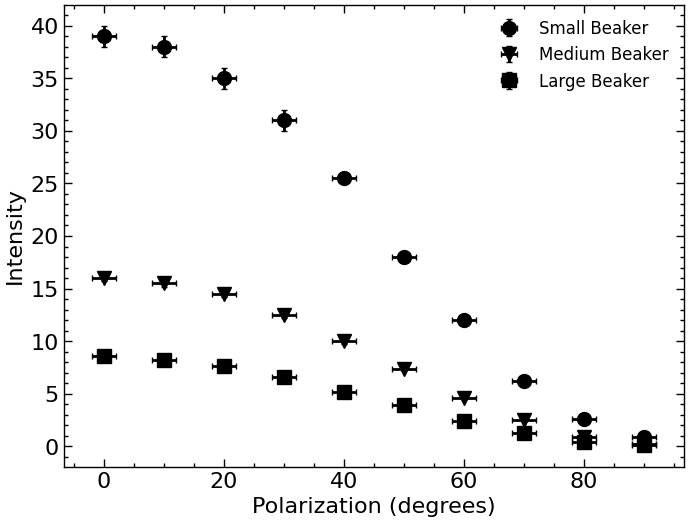
\includegraphics[width=\columnwidth]{../figures/water.png}
    \end{center}
    \caption{Intensity vs. Polarization for varying beaker sizes with water. Here, the polarization is measured in degrees and the intensity is measured in arbitrary units.}
    \label{fig:water}
\end{figure}

\begin{figure}[H]
    \begin{center}
        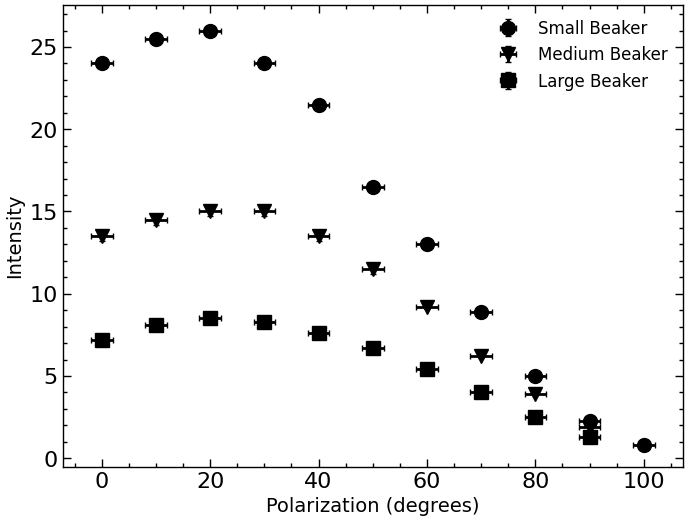
\includegraphics[width=\columnwidth]{../figures/solution1.png}
    \end{center}
    \caption{Intensity vs. Polarization for varying beaker sizes with solution 1. Here, the polarization is measured in degrees and the intensity is measured in arbitrary units.}
    \label{fig:solution1}
\end{figure}

\begin{figure}[H]
    \begin{center}
        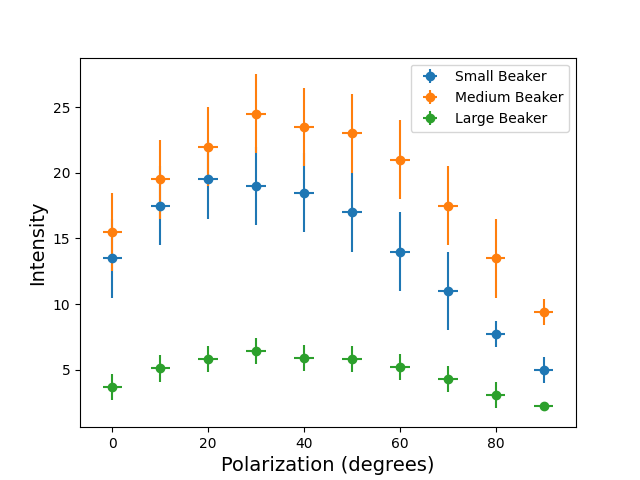
\includegraphics[width=\columnwidth]{../figures/solution2.png}
    \end{center}
    \caption{Intensity vs. Polarization for varying beaker sizes with solution 2. Here, the polarization is measured in degrees and the intensity is measured in arbitrary units.}
    \label{fig:solution2}
\end{figure}

\begin{figure}[H]
    \begin{center}
        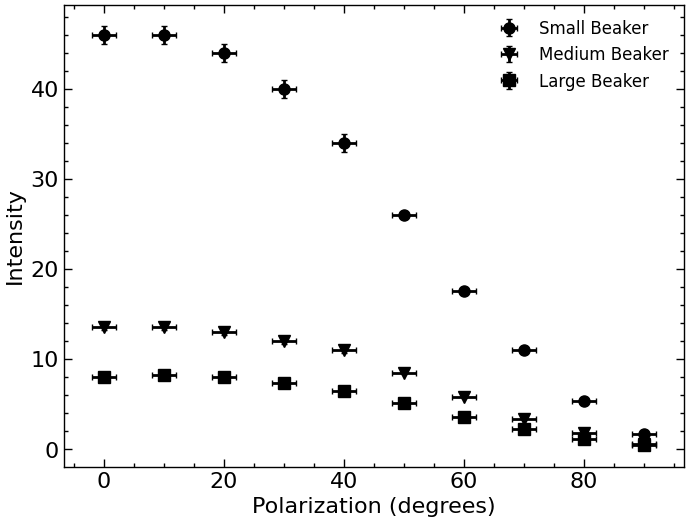
\includegraphics[width=\columnwidth]{../figures/solution3.png}
    \end{center}
    \caption{Intensity vs. Polarization for varying beaker sizes with solution 3. Here, the polarization is measured in degrees and the intensity is measured in arbitrary units.}
    \label{fig:solution3}
\end{figure}

\begin{figure}[H]
    \begin{center}
        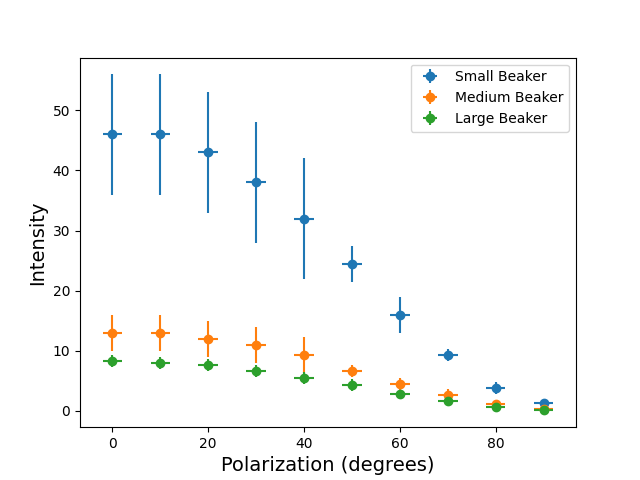
\includegraphics[width=\columnwidth]{../figures/solution4.png}
    \end{center}
    \caption{Intensity vs. Polarization for varying beaker sizes with solution 4. Here, the polarization is measured in degrees and the intensity is measured in arbitrary units.}
    \label{fig:solution4}
\end{figure}

\newpage
Each of the following graphs show the phase shift as a function of sugar concentration in water, with each separate graph containing data from one beaker size. 
The phase shifts were found by fitting the intensity vs. polarization data to a cosine function in the form $A\cos{\left(Bx+C\right)}+D$. We invoked the ODR (orthogonal distance regression) class from the SciPy Python package to fit these data sets to the previously mentioned cosine function. By representing phase shift versus sugar concentration, we can quantify how the polarization of light changes as a function of sugar concentration in water.

\begin{figure}[H]
    \begin{center}
        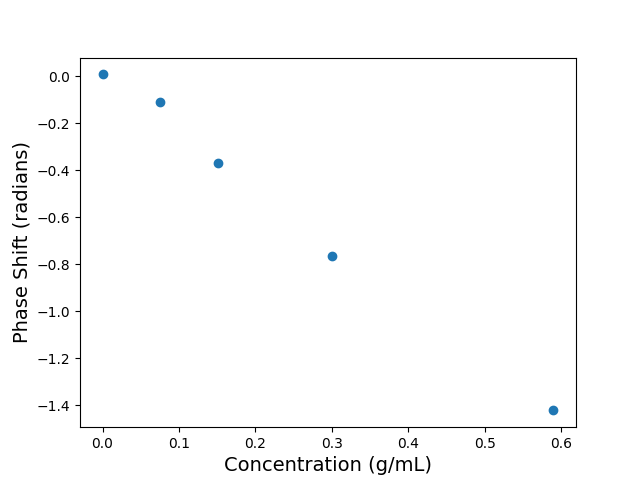
\includegraphics[width=\columnwidth]{../figures/large_beaker_phase_shifts.png}
    \end{center}
    \caption{This graph shows the phase shifts for the large beaker.}
    \label{fig:large_beaker_phase_shifts}
\end{figure}

\begin{figure}[H]
    \begin{center}
        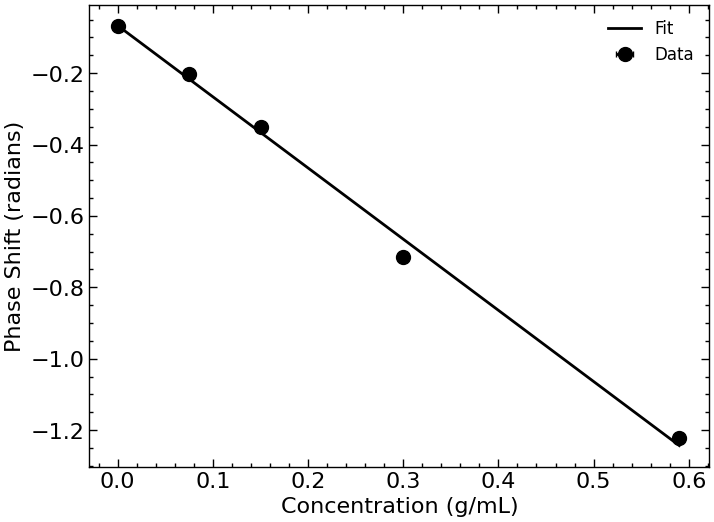
\includegraphics[width=\columnwidth]{../figures/medium_beaker_phase_shifts.png}
    \end{center}
    \caption{Phase shifts for medium beaker.}
    \label{fig:medium_beaker_phase_shifts}
\end{figure}

\begin{figure}[H]
    \begin{center}
        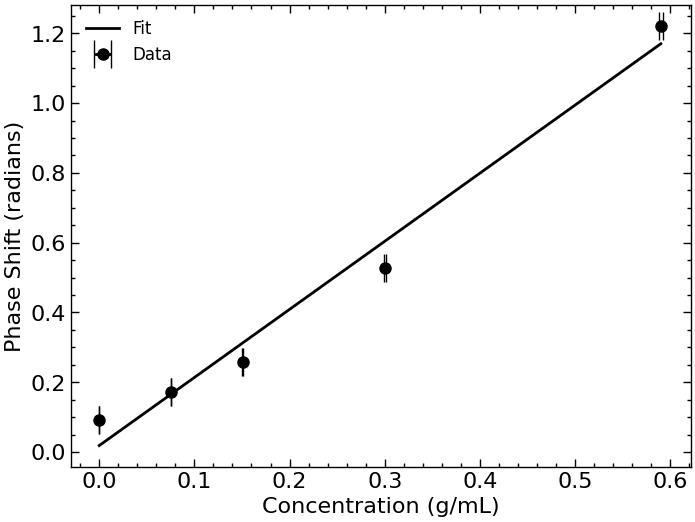
\includegraphics[width=\columnwidth]{../figures/small_beaker_phase_shifts.png}
    \end{center}
    \caption{Phase shifts for small beaker.}
    \label{fig:small_beaker_phase_shifts}
\end{figure}

\begin{figure}[H]
	\begin{center}
		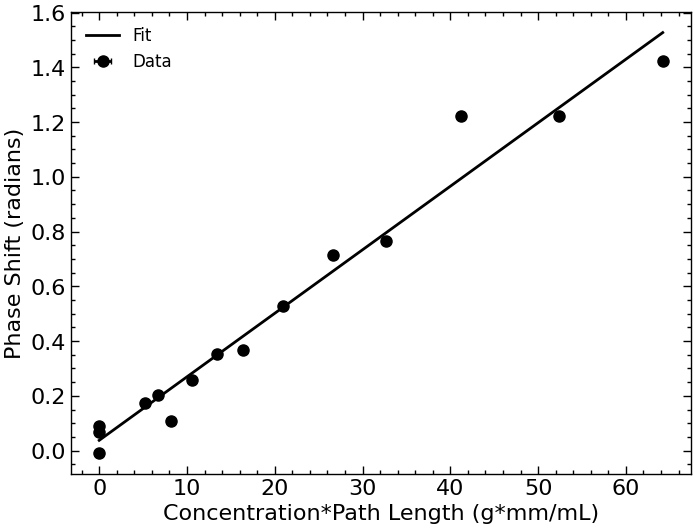
\includegraphics[width=\columnwidth]{../figures/concentration_times_diameter_phase_shifts.png}
	\end{center}
	\caption{This figure encapsulates the phase shift in radians as a function of both concentration in grams per milileter and the path length in milimeters, where the horizontal axis is the product of the concentration and path length values.}
	\label{fig:concentration_times_diameter_phase_shifts}
\end{figure}